% ----------------------------------------------------------------------------
% O básico de um \external
% ----------------------------------------------------------------------------

\chapter{O básico de um \external}

Escrever um \external significa seguir as recomendações da API. Peço ao leitor
bastante paciência pois este tutorial pretende andar um pouco devagar para
mostrar os passos da escrita de um \external.

% -----+-----+-----+-----+-----+-----+-----+-----+-----+-----+-----+-----+-----+
%      |     |     |     |     |     |     |     |     |     |     |     |     |
% -----+-----+-----+-----+-----+-----+-----+-----+-----+-----+-----+-----+-----+
\section{Um \external Hello World}

Como dissemos anteriormente, a arquitetura do Pure Data é organizada de acordo
com o paradigma de orientação a objetos: cada objeto gráfico do Pure Data
corresponde a uma instância de uma classe. Neste sentido, um \external está
associado a um conjunto de estruturas de dados que representam classes em C.
Veja que o conceito de objeto aqui não remete ao conceito de objetos de
linguagens de programação como Java ou C++.
Para cada classe é necessário haver métodos de instanciação, destruição,
processamento de sinais, tratamento de mensagens, etc.

A infraestrutura mínima para o funcionamento de um \external (de nome, digamos,
\texttt{<external>}) consiste em uma estrutura de dados para a representação
de uma classe, que deve ter nome \texttt{t\_<external>}, e dois métodos
obrigatórios, chamados \texttt{<external>\_setup()} e
\texttt{<external>\_new()}. Note que a convenção de nomes utilizada no Pure
Data é de que toda função deve ser nomeada da forma
\texttt{<contexto>\_<funcao>()}.

A estutura de dados que representa uma classe do Pure Data deve
obrigatoriamente possuir o primeiro atributo do tipo \texttt{t\_object}, no
qual é armazenado o objeto criado no momento da instanciação.
Outros atributos podem ser adicionados a esta estrutura de maneira que cada
instância da mesma classe possua os atributos necessários para seu
funcionamento.
Uma classe que acessa um arquivo, por exemplo, pode possuir como atributos uma
string para guardar o caminho e um inteiro para guardar o descritor do
arquivo.

Um exemplo de estrutura de dados para representação de uma classe chamada
\texttt{helloworld} consiste no seguinte:

\vspace{1em}
\begin{lstlisting}[caption=Estruturas de dados de um \external]
// ---------------------------------------------------
// Class definition
// ---------------------------------------------------
static t_class *helloworld_class;

// ---------------------------------------------------
// Data structure definition
// ---------------------------------------------------
typedef struct _helloworld {
   t_object x_obj;
} t_helloworld;
\end{lstlisting}

Tal objeto é passado para as funções que tratam mensagens e por isto tudo o que
for necessário para o funcionamento de seu external deve estar contido neste
objeto.
Aproveitamos para recomendar que isto inclua toda alocação e liberação de
memória que possa ser necessária.

Sempre que um \external é carregado pelo Pure Data, o método de nome
\texttt{<external>\_setup()} é executado. No exemplo dado acima, o Pure
Data irá procurar, no arquivo binário \texttt{example1.pd\_linux} que contém
a biblioteca compartilhada, o método de nome \texttt{example1\_setup(void)}.
Este método é utilizado para realizar a inicialização da classe, informando ao
Pure Data da existência de uma nova classe no sistema e associando a ela os
métodos de instanciação e destruição, além de outras informações:

\vspace{1em}
\begin{lstlisting}[caption=Método setup]
void helloworld_setup(void) {
   helloworld_class = class_new(
      gensym("helloworld"),          // Nome simbolico
      (t_newmethod) helloworld_new,  // Construtor
      (t_method) helloworld_destroy, // Destrutor
      sizeof (t_helloworld),         // Tamanho do objeto
      CLASS_NOINLET,                 // Flags com o tipo da classe
      0);                            // Argumentos do construtor
}
\end{lstlisting}

Dentro do método \texttt{<external>\_setup()} não há limite para o número de
classes a definir, de forma que é possível definir apenas uma classe (como no
exemplo helloworld.c) ou uma biblioteca inteira com várias classes (como no exemplo 3).
A introdução de uma nova classe no sistema é realizada pela função
\texttt{class\_new()}.
São parâmetros da função \texttt{class\_new()}:

\begin{itemize}
\item Nome simbólico da classe.
\item Método construtor de um objeto.
\item Método destrutor de um objeto.
\item Tamanho do espaço de dados dos atributos de um objeto.
\item Flags que definem a representação gráfica do objeto.
\item Tipos dos parâmetros a serem passados para o construtor quando da
      instanciação de um objeto (veja o próximo capítulo).
\end{itemize}

Os tipos de Flags aceitas para representar um objeto são:
\begin{itemize}
   \item CLASS\_DEFAULT - Para objetos padrões do PD com 1 inlet
   \item CLASS\_NOINLET - Objetos sem inlet ``Mágico''
   \item CLASS\_PD - Para objetos sem representação gráfica, como inlets
   \item CLASS\_GOBJ - Para objetos gráficos como arrays e graphs
   \item CLASS\_PATCHABLE - Para objetos internos do PD como ``message'' ou ``text''
\end{itemize}

É necessário terminar a lista de tipos de parâmetros com um número inteiro 0,
para indicar ao Pure Data que a lista de tipos terminou.
Consulte a documentação da função \texttt{class\_new()} para mais
detalhes\footnote{\url{http://pdstatic.iem.at/externals-HOWTO/node9.html\#SECTION00092100000000000000}}.

O método \texttt{<external>\_new()}, que foi associado como método de
instanciação de objetos na chamada de \texttt{class\_new()}, realiza a
instanciação de objetos propriamente dita.
Neste método, além da instanciação de um novo objeto através da função
\texttt{pd\_new()}, é possível definir os
valores dos atributos da estrutura de dados da classe e também inicializar
quaisquer outros contextos que sejam necessários, como por exemplo abrir
arquivos, preencher vetores, alocar memória, etc.

\vspace{1em}
\begin{lstlisting}[caption=Construtor de uma classe]
// ---------------------------------------------------
// Construtor da classe
// ---------------------------------------------------
void * helloworld_new(void){
   t_helloworld *x = (t_helloworld *) pd_new(helloworld_class);
   // Something else?
   return (void *) x;
}
\end{lstlisting}

Após a criação da estrutura de dados dos métodos da forma mencionada acima, a
compilação realizada da forma descrita na seção \ref{sec:compiling}, e a
criação do objeto no Pure Data como descrito na seção \ref{sec:using}, o
resultado pode ser visto na figura \ref{fig:example01working}.

\begin{figure}[h!]
  \centering
  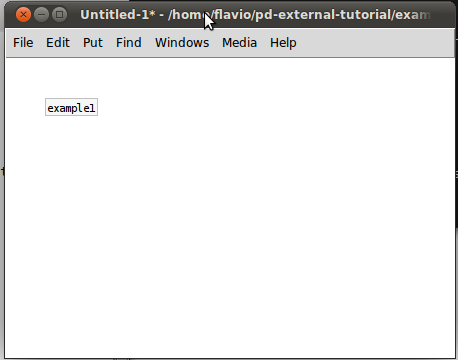
\includegraphics[scale=\Mysize]{example1}
  \caption{Nosso primeiro \external do PD. Ainda inútil. :-$\left.\right)$}
  \label{fig:example01working}
\end{figure}

% -----+-----+-----+-----+-----+-----+-----+-----+-----+-----+-----+-----+-----+
%      |     |     |     |     |     |     |     |     |     |     |     |     |
% -----+-----+-----+-----+-----+-----+-----+-----+-----+-----+-----+-----+-----+
\section{Uma biblioteca simples}

Um mesmo método \texttt{<external>\_setup()} pode definir várias classes
diferentes. A isto damos o nome de biblioteca. Neste cenário, o método
\texttt{<external>\_setup()} possui o mesmo nome do arquivo com a biblioteca,
mas cada classe podem ter um nome diferente (veja o exemplo 3).

\vspace{1em}
\begin{lstlisting}[caption=Exemplo de arquivo com duas classes]
void example3_setup(void) {
  post("Initializing my library");

  myobj1_class = class_new(
    gensym("myobj1"),
    (t_newmethod) myobj1_new, // Constructor
    0,
    sizeof (t_myobj1),
    CLASS_NOINLET,
    0);
  class_sethelpsymbol(myobj1_class, gensym("myobj1-help"));

  myobj2_class = class_new(
    gensym("myobj2"),
    (t_newmethod) myobj2_new, // Constructor
    0,
    sizeof (t_myobj2),
    CLASS_NOINLET,
    0);
  class_sethelpsymbol(myobj2_class, gensym("myobj2-help"));
}
\end{lstlisting}

Se o arquivo foi preenchido corretamente, compilado corretamente e adicionado
ao caminho do PureData, teremos o resultado visto na figura \ref{fig:exemplo3}.

\begin{figure}[h!]
	\centering
	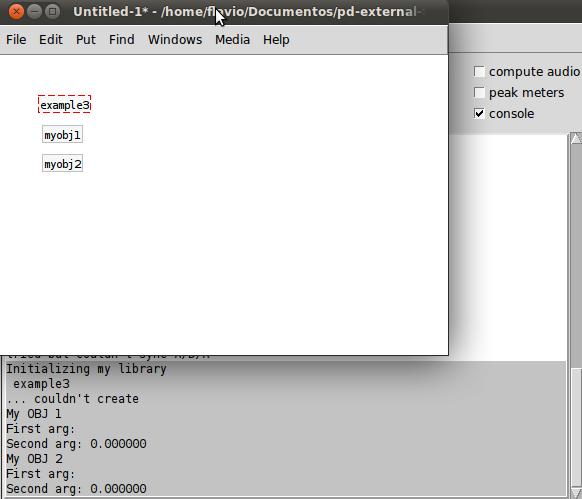
\includegraphics[scale=\Mysize]{example3}
	\caption{Nosso segundo \external do PD. Ainda inútil. :-$\left.\right)$}
        \label{fig:exemplo3}
\end{figure}

Apesar de este tipo de biblioteca ser bastante utilizado no código-fonte do PD,
é recomendado separar os \external em arquivos individuais para simplificar
a leitura e manutenção do código-fonte.
Sendo assim, é recomendado que o \external ``myobj1'' esteja em um arquivo
chamado ``myobj1.c'' e que o mesmo seja feito com o \external ``myobj2''.

Dentro do Pure Data, um clique com o botão direito em um objeto abre um menu
no qual uma das opções é \texttt{Ajuda}. Quando esta opção é selecionada, o
Pure Data abre um patch associado ao objeto, que deve conter instruções e
exemplos de uso. Por padrão, o Pure Data procura um arquivo com o mesmo nome
que o external (acrescido da extensão \texttt{-help.pd}) no diretório padrão de
documentação (\texttt{doc/5.reference}). Para associar um arquivo diferente do
padrão, basta utilizar a função \texttt{class\_sethelpsymbol}:

\vspace{1em}
\begin{lstlisting}[caption=Definição de arquivo de help]
class_sethelpsymbol(myclass_class, gensym("my_class-help"));
\end{lstlisting}

Um objeto pode ainda ter outros nomes (\emph{aliases}). Para definir isto
podemos utilizar a função \texttt{class\_addcreator()}. Veja o exemplo:

\vspace{1em}
\begin{lstlisting}[caption=Definição de alias para um objeto]
class_addcreator((t_newmethod)medusa_new, gensym("med"), 0);
\end{lstlisting}

Exemplos comuns de aliases são os objetos [send], [receive] e [trigger], que
podem ser instanciados pelos aliases [s], [r] e [t] respectivamente.

% -----+-----+-----+-----+-----+-----+-----+-----+-----+-----+-----+-----+-----+
%      |     |     |     |     |     |     |     |     |     |     |     |     |
% -----+-----+-----+-----+-----+-----+-----+-----+-----+-----+-----+-----+-----+
\section{Variáveis globais}

É possível utilizar variáveis globais para armazenar dados de um \external.
Estas variáveis são visíveis para todas as intâncias de objetos do \external e
todas podem alterar seus valores.
Isto pode ser útil ou um desastre (veja o exemplo16).
Por exemplo, cada instância do \external \texttt{example16}
definido a partir do código a seguir incrementa em uma unidade o valor do
contador, como pode ser visto na figura \ref{fig:counter}:

\vspace{1em}
\begin{lstlisting}[caption=Exemplo de uma variável global]
int count = 0;

void * example16_new(void) {
    t_example16 *x = (t_example16 *) pd_new(example16_class);
    post("Counter value: %d",count);
    count++;
    return (void *) x;
}
\end{lstlisting}

\begin{figure}[h!]
  \centering
  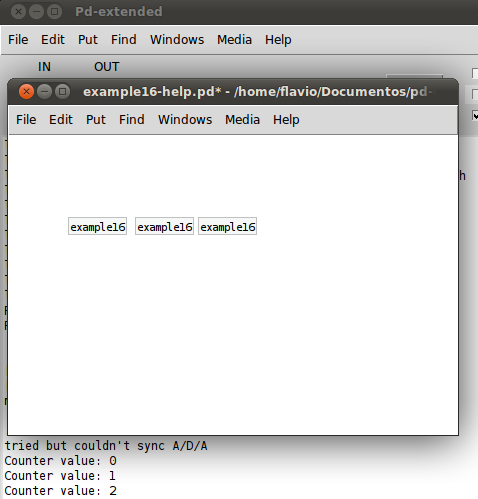
\includegraphics[scale=\Mysize]{example16}
  \caption{Repare na saída da janela principal.}
  \label{fig:counter}
\end{figure}

Caso isto não seja desejável, o ideal é incluir as variáveis dentro da
estrutura do objeto.
Assim, neste exemplo cada instância terá seu próprio contador:

\vspace{1em}
\nopagebreak{
\begin{lstlisting}[caption=Objeto contador]
static t_class *counter_class;

typedef struct _counter {
   t_object x_obj;
   t_float counter;
   t_outlet * x_outlet_output_float;
} t_counter;

void * counter_new(void){
   t_counter *x = (t_counter *) pd_new(counter_class);
   x->counter = 0;
   x->x_outlet_output_float = outlet_new(&x->x_obj, gensym("float"));
   return (void *) x;
}
\end{lstlisting}

Vale notar que adicionar a estrutura de dados do \external os atributos
necessários para seu funcionamento é a abordagem padrão para o desenvolvimento.
É recomendado que o compartilhamento de dados entre dois objetos ocorra pela
troca de mensagem e não por variáveis globais.


